%================ NOTEBOOK APPLICATION ================
\chapter{Notebook Application: A NotebookLM-Style Front End}\label{ch:notebook}

\section{Motivation and scope}
The service of Chapter~\ref{ch:service} answers questions through an API. To make the abstention-aware agent usable by people who are not developers, we built a web application modelled on Google NotebookLM: a user collects sources in a \emph{notebook}, asks questions about them, and turns them into study and briefing material. The application keeps the project's central property visible: every answer is cited, and when the sources do not contain the answer the assistant says so instead of guessing. The front end has about 3{,}300 lines of TypeScript (Next.js~16, React~19, Tailwind~4); the notebook features added about 3{,}000 lines of Python, including tests, to the service. It was built and delivered in five phases.

\begin{figure}[H]
\centering
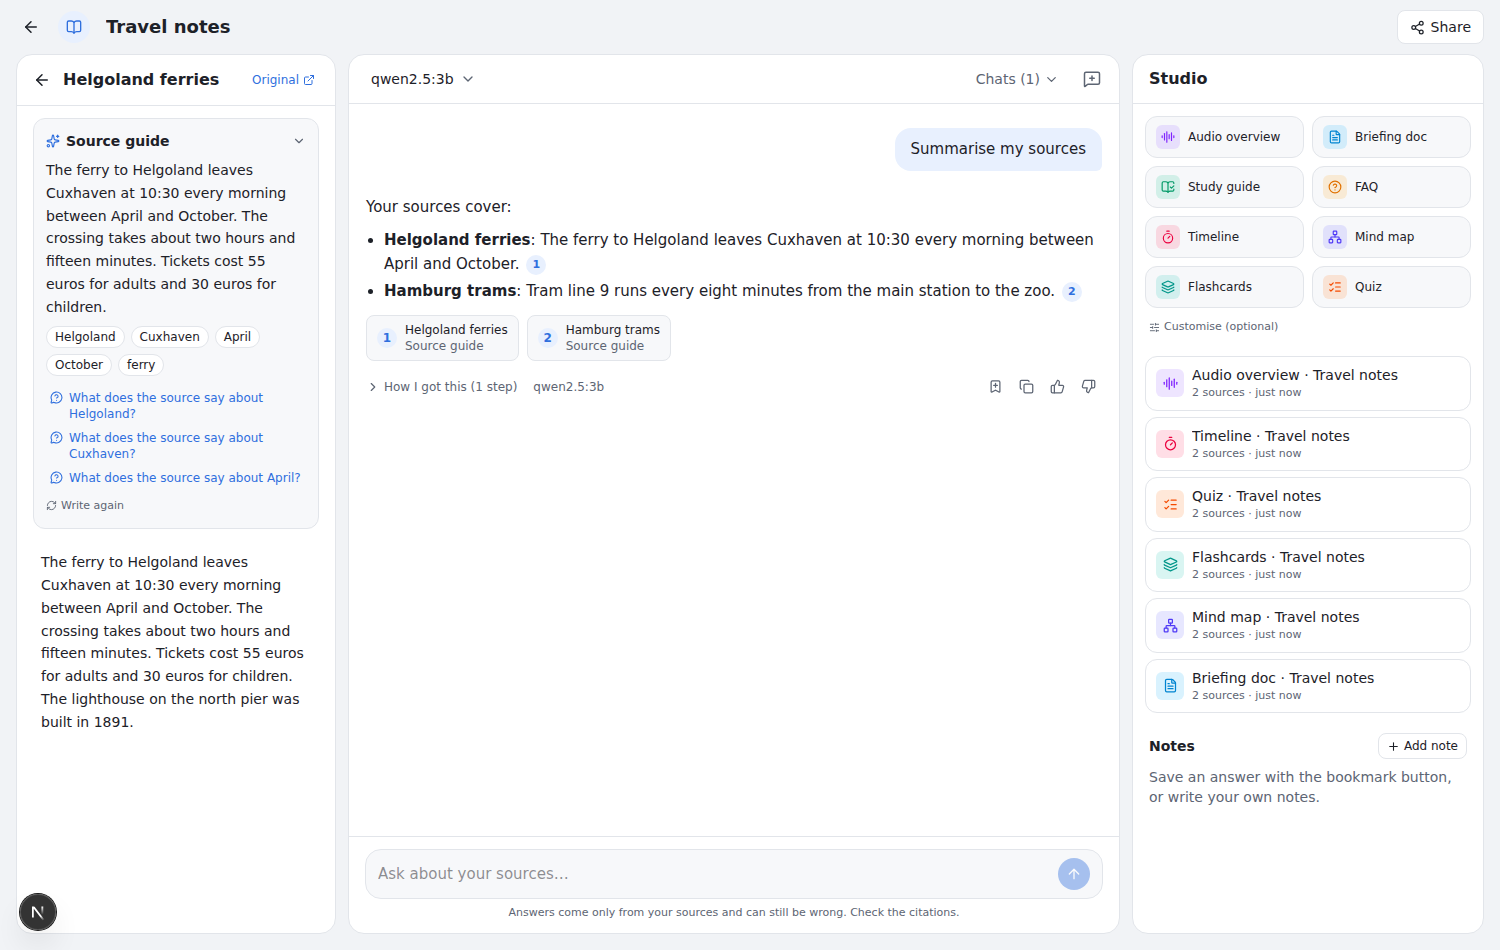
\includegraphics[width=\textwidth]{fig_ui_notebook.png}
\caption{A notebook: sources with a source guide (left), a notebook-wide question answered from the source guides with one citation per source (middle), and the Studio with generated outputs (right). Screenshot from the development mode, in which a scripted stand-in replaces the LLM.}
\label{fig:ui_notebook}
\end{figure}

\section{Features}
\begin{table}[H]
\centering\small
\begin{tabularx}{\textwidth}{@{}p{2.3cm}Y@{}}
\toprule
Part & What it does \\
\midrule
Sources & Files (PDF, Word, HTML, Markdown, text), web pages, YouTube videos (their transcript), pasted text, and web search (``discover sources''). Each source can be ticked in or out of the answers and read in a viewer by section and page; citations open the viewer at the cited passage, and YouTube citations open the video at the cited minute. \\
Source guide & For every source the LLM writes a short summary, five key topics and three questions the source answers; clicking a question asks it in the chat. \\
Chat & Streamed, cited answers from the S5 agent with an evidence meter (1 $-$ P(unanswerable)), the agent's steps, the model used, feedback, copy and save-to-notes. Questions about the whole notebook are answered from the source guides (Section~\ref{sec:overview}). \\
Studio & Audio overview (two hosts, spoken by Kokoro), briefing document, study guide, FAQ, timeline, mind map, flashcards and quiz, generated from the ticked sources with optional instructions; plus notes. \\
Model menu & Every available model, grouped into standard and thinking models, with size, speed and a shield for calibrated refusal thresholds (Section~\ref{sec:permodel}). \\
Sharing & Notebooks can be shared with people as viewer or editor, or with anyone signed in who has the link. \\
\bottomrule
\end{tabularx}
\caption{Features of the notebook application.}
\label{tab:notebook}
\end{table}

\section{Architecture}
The browser talks only to the FastAPI service. Slow work runs in the Celery worker: fetching web pages and transcripts, indexing, writing source guides, generating Studio outputs and speaking audio overviews. The front end polls while work is in progress. Four database migrations added source types and guides (\texttt{0003}), Studio outputs (\texttt{0004}) and sharing (\texttt{0005}) after the notes table (\texttt{0002}).

\begin{figure}[H]
\centering
\begin{tikzpicture}[every node/.style={font=\small, align=center}, box/.style={draw, rounded corners=3pt, fill=gray!8, minimum height=0.95cm, minimum width=2.4cm, inner sep=3pt}, ar/.style={-{Stealth[length=6pt]}, thick}]
\node[box, fill=blue!8] (ui) at (0,0) {Next.js\\notebook UI};
\node[box, fill=orange!15, minimum width=3.0cm] (api) at (3.9,0) {FastAPI\\roles, SSE};
\node[box, fill=green!10] (ag) at (8.0,1.0) {S5 agent /\\overview answer};
\node[box] (wk) at (8.0,-1.0) {Celery worker\\fetch, index, guide,\\Studio, speech};
\node[box] (llm) at (12.2,1.4) {LLM\\(chosen model)};
\node[box] (tts) at (12.2,0.0) {Kokoro TTS};
\node[box] (web) at (12.2,-1.4) {Web, YouTube,\\search};
\draw[ar] (ui)--(api);
\draw[ar] (api)--(ag); \draw[ar] (api)--(wk);
\draw[ar] (ag)--(llm); \draw[ar] (wk)--(llm); \draw[ar] (wk)--(tts); \draw[ar] (wk)--(web);
\end{tikzpicture}
\caption{The notebook application on top of the service.}
\label{fig:notebook_arch}
\end{figure}

\section{Sources beyond files}
\begin{itemize}
\item \textbf{Web pages} are downloaded by the worker (HTML, PDF or plain text, up to the upload size limit) and indexed like an uploaded file. Because the server fetches a URL given by a user, every address and every redirect target is resolved and refused if it points to a private, loopback or link-local network (protection against server-side request forgery). Stored pages are only served as downloads with a sandboxing content-security policy, so a fetched page can never run scripts on the API's origin.
\item \textbf{YouTube videos} become their transcript, grouped into two-minute sections whose headings are timestamps (``4:00''); the section-aware chunker of Chapter~\ref{ch:service} keeps these as contextual headers, so a citation knows its minute and opens the video there.
\item \textbf{Pasted text} is stored as a Markdown file.
\item \textbf{Discover sources} searches the web for a topic (DuckDuckGo without a key, or Tavily, Brave or SearXNG) and adds the results the user ticks.
\end{itemize}

\section{Source guides and notebook-wide questions}\label{sec:overview}
The agent retrieves five passages for a question. That works for specific questions but not for questions about the whole notebook, such as ``summarise my sources'' or ``what are the main themes?'': five passages cover only part of the material, and the gate would often (correctly, for those passages) judge the evidence weak. After a source is indexed, the worker therefore writes a \emph{source guide} from an even sample of its passages (beginning, middle and end, about 6{,}000 characters). Questions recognised as notebook-wide are answered from the guides of the ticked sources, and the answer cites each source; all other questions still go through retrieval, the gate and the self-check. The answer passes through the same output guardrails as the agent's answers.

\section{Studio outputs}
Each Studio output is one LLM call over a numbered digest of the ticked sources (each source's guide summary plus spread excerpts, about 7{,}000 characters in total, which fits a 4k-token context with room for the answer). Small local models follow simple labelled formats much more reliably than JSON, so each kind asks for a fixed plain-text layout that a lenient parser turns into structured data; if the parse finds nothing, the output is marked failed rather than shown broken.

\begin{table}[H]
\centering\small
\begin{tabularx}{\textwidth}{@{}p{2.5cm}p{5.2cm}Y@{}}
\toprule
Output & Format asked from the LLM & Shown as \\
\midrule
Briefing doc & Markdown sections: summary, key points, details, open questions & Document with clickable source numbers \\
Study guide & Concepts, 5 short-answer questions, answer key, essay questions & Document \\
FAQ & \texttt{Q:} / \texttt{A:} pairs & Question--answer list \\
Timeline & \texttt{date | event [n]}, or ``NO DATES'' & Vertical timeline with sources \\
Mind map & Indented list & Interactive tree: fold branches, click a topic to ask about it \\
Flashcards & \texttt{Q: \ldots{} | A: \ldots{} [n]} & Flip cards with shuffle \\
Quiz & Question, options A--D, \texttt{ANSWER:}, \texttt{WHY:} & Scored quiz with explanations \\
Audio overview & \texttt{ALEX:} / \texttt{SAM:} turns & Audio player and script \\
\bottomrule
\end{tabularx}
\caption{Studio outputs.}
\label{tab:studio}
\end{table}

\begin{figure}[H]
\centering
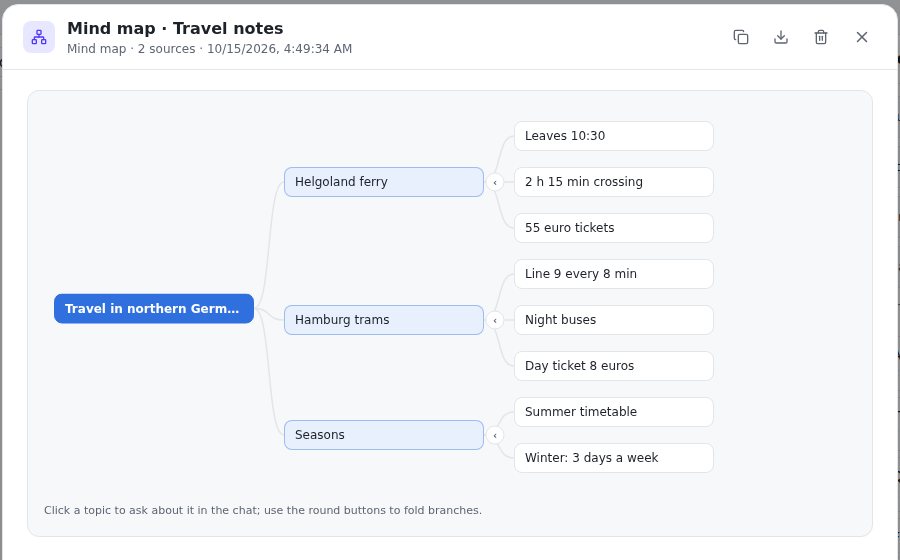
\includegraphics[width=0.8\textwidth]{fig_ui_mindmap.png}
\caption{An interactive mind map generated from two sources (development mode).}
\label{fig:ui_mindmap}
\end{figure}

\textbf{Audio overview.} The script's turns are spoken by Kokoro-82M, an open-weight text-to-speech model served on the CPU by Kokoro-FastAPI in its own container, with a different voice for each host. The service requests raw 16-bit audio for each turn and joins the turns into one WAV file with short pauses. If the voice service is not running, the script is still saved and shown, and the user can have it spoken later.

\section{Choosing the model}
Like the model menus of ChatGPT and Claude.ai, the user picks the model per message from every model available: the models installed in Ollama on the laptop and, when an API key is set, every model of OpenRouter, OpenAI, Anthropic, Google, Groq, Mistral, DeepSeek or Together, listed live from each provider. The menu groups models by ability into \emph{standard models}, which answer directly, and \emph{thinking models} (DeepSeek-R1, Qwen3, OpenAI's o-series), which reason before answering. For thinking models the service hides the reasoning text, raises the output budget to 4{,}000 tokens and the time limit to 10 minutes. We installed ten free open-weight models of 1--4 billion parameters that fit the 4\,GB GPU.

\begin{figure}[H]
\centering
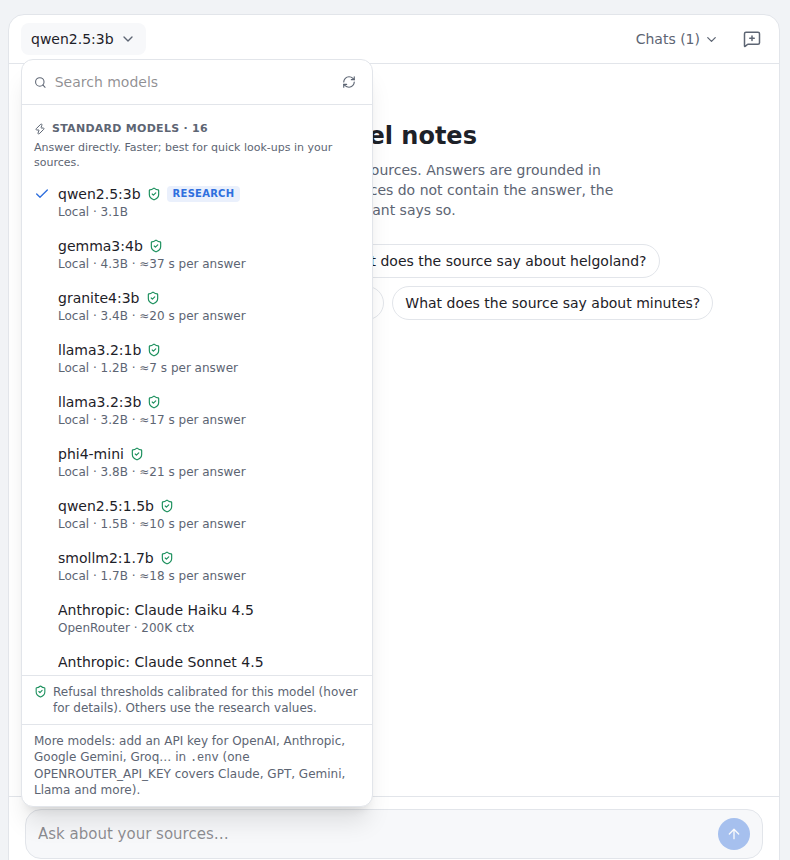
\includegraphics[width=0.55\textwidth]{fig_ui_models.png}
\caption{The model menu: standard models with size, measured speed and the calibration shield (development mode, with a sample cloud catalogue).}
\label{fig:ui_models}
\end{figure}

\section{Refusal thresholds for every model}\label{sec:permodel}
The abstention thresholds of Chapter~\ref{ch:agent} were tuned for Qwen2.5-3B: the agent abstains when the gate score $p \ge \tau$, when the generator refuses, or when $p \ge$ min\_p and the self-check judges the answer unsupported. The gate does not depend on the LLM, but how often a model refuses on its own and how strict its self-check is do. We therefore calibrated $\tau$ and min\_p \textbf{per model}, on the same 224 MTRAG development examples used for the research calibration (150 answerable, 74 unanswerable; never the test set). Each model answered every example through the service's own client, and the self-check judged every answer. A grid search then chose the pair with the best abstention F1 among those whose false-abstention rate is at most the model's own refusal rate plus 10 points (the research procedure allowed 5 points for the gate and 5 for the self-check). Qwen2.5-3B keeps its research values, so the earlier chapters stay valid. The service applies each model's own thresholds to every answer and records them with it.

\begin{table}[H]
\centering\small
\begin{tabular}{@{}lrrrrrrr@{}}
\toprule
Model & $\tau$ & min\_p & F1 & Recall & FA & Own refusals & s / question \\
\midrule
gemma3:4b & .64 & .55 & \textbf{.67} & .85 & .34 & .33 & 37 \\
qwen3:1.7b (thinking) & .63 & .35 & \textbf{.67} & .72 & .21 & .15 & 32 \\
granite4:3b & .61 & .45 & .64 & .88 & .43 & .38 & 20 \\
qwen2.5:3b (research) & .61 & .50 & .62 & .73 & .30 & .22 & -- \\
llama3.2:3b & .45 & .35 & .62 & .89 & .48 & .38 & 17 \\
phi4-mini (3.8B) & .52 & off & .60 & .92 & .57 & .54 & 21 \\
qwen2.5:1.5b & .61 & .35 & .56 & .49 & \textbf{.12} & .02 & 10 \\
smollm2:1.7b & .61 & .50 & .54 & .46 & \textbf{.12} & .02 & 18 \\
deepseek-r1:1.5b (thinking) & .54 & off & .54 & .51 & .19 & .09 & 38 \\
llama3.2:1b & .52 & off & .53 & .72 & .48 & .38 & 7 \\
\bottomrule
\end{tabular}
\caption{Per-model calibration on the MTRAG development examples. FA: answerable questions refused with the chosen thresholds; own refusals: refused by the model alone, with no gate and no self-check. Times include the answer and the self-check on the GTX~1650.}
\label{tab:permodel}
\end{table}

\begin{itemize}
\item \textbf{No model is best on every measure.} Gemma-3-4B and Qwen3-1.7B have the best F1, but Gemma refuses a third of the answerable questions by itself, while Qwen3-1.7B refuses only 21\% in total: it is the best balance and better than the research model.
\item \textbf{Models differ mostly in their own refusals.} Phi-4-mini refuses 54\% of answerable questions before the gate acts; Qwen2.5-1.5B and SmolLM2 almost never refuse, so the gate does nearly all of their abstaining and their recall is low.
\item \textbf{The best thresholds differ by model} ($\tau$ from .45 to .64; the self-check is switched off for three models), which shows why one set of thresholds cannot serve every model.
\item \textbf{Hardware limits.} Qwen3-4B needed about seven minutes per question with its reasoning partly on the CPU; the calibration (and normal use) was impractical on the 4\,GB GPU, so it was removed.
\end{itemize}
These are development-set results for a single run per model; they guide the choice of model in the application but are not test-set results.

\section{End-to-end test on research papers}\label{sec:smoke}
To check the finished application as a user meets it, a test script (\texttt{scripts/smoke\_test.py}) drives the running service exactly as the interface does, for every installed model. It uploads three research papers (QPolypNet, 86 passages; NQNN, 53 passages; a two-page extended abstract on end-to-end encoders for QCNNs, 12 passages) and checks, once: indexing, source guides, section headings, file download, pasted text, a web page, Discover, notes and sharing. Then, for each model, it asks three questions per paper: a general one (\emph{What problem does this paper address\dots?}), a section question (\emph{Explain the experiments\dots and their main results}) and an unanswerable one (\emph{What was the weather in the city where the authors live on the day the paper was submitted?}). It also asks a follow-up in the same chat (\emph{What limitations does it mention?}), two notebook-wide questions, and generates a FAQ and flashcards; the first model also produces an audio overview. The whole run took 111 minutes on the GTX~1650.

\textbf{Every feature worked with every model}: 184 checks, 162 passed, 22 warnings and no failures. A warning means the service worked but the model's decision was not the ideal one (for example, it answered the unanswerable question); these are the behaviours this project measures, not faults.

\begin{table}[H]
\centering\small
\begin{tabular}{@{}lccccr@{}}
\toprule
Model & Unanswerable & Answerable & Wrong refusals by & Follow-up & Median s \\
 & refused & answered & & & \\
\midrule
gemma3:4b & 3/3 & 6/6 & -- & clarify & 72 \\
granite4:3b & 3/3 & 6/6 & -- & clarify & 37 \\
llama3.2:3b & 3/3 & 6/6 & -- & clarify & 33 \\
llama3.2:1b & 3/3 & 6/6 & -- & answered & 21 \\
qwen3:1.7b (thinking) & 3/3 & 5/6 & gate & clarify & 35 \\
phi4-mini & 3/3 & 5/6 & generator & refused & 46 \\
qwen2.5:1.5b & 3/3 & 5/6 & gate & answered & 23 \\
qwen2.5:3b (research) & 3/3 & 1/6 & self-check (4), generator & clarify & 31 \\
deepseek-r1:1.5b (thinking) & \textbf{1/3} & 4/6 & gate (2) & answered & 24 \\
smollm2:1.7b & \textbf{1/3} & 4/6 & gate (2) & answered & 22 \\
\midrule
All & 26/30 & 48/60 & & & \\
\bottomrule
\end{tabular}
\caption{End-to-end test on three research papers. Answerable: the general and the section question on each paper. Wrong refusals: which part of the agent refused an answerable question. Median s: time per chat question, including retrieval, gate, answer and self-check.}
\label{tab:smoke}
\end{table}

\begin{itemize}
\item \textbf{Hallucination follows the model's own refusal rate.} The four answered unanswerable questions came from DeepSeek-R1-1.5B and SmolLM2-1.7B, the two models that almost never refuse on their own in the calibration (Table~\ref{tab:permodel}: 9\% and 2\%). Both ``answered'' the weather question and cited the introduction. Of the 26 correct refusals, 13 came from the gate and 13 from the generator itself: the gate score for the weather question ranged from 0.29 to 0.81, because the retrieved passages are on the paper's topic. The gate alone is therefore not enough for such questions, and a model that refuses on its own adds real protection.
\item \textbf{Domain shift moves the gate.} Six of the twelve wrong refusals were made by the gate, with $p$ between 0.55 and 0.73 on general and experiments questions. The gate was trained on MTRAG's conversational domains (Wikipedia, finance, government, cloud documentation); dense scientific text with tables and equations raises its estimate that a question is unanswerable. This is the same drift the project studies across conversation turns, here across domains, and it suggests calibrating the gate on documents like the user's.
\item \textbf{The research model is the most cautious.} Qwen2.5-3B refused five of six answerable questions, four of them through the self-check with $p$ between 0.51 and 0.61, inside its self-check band ($\text{min\_p}=0.50 \le p < \tau=0.61$). Its self-check judges answers about technical papers as unsupported more often than the other models do, so for papers a model such as Gemma-3-4B or Llama-3.2-3B is the better choice in the application.
\item \textbf{Follow-ups.} Four models answered the follow-up from the papers' conclusions; five asked which paper or which limitations were meant. Asking is the right behaviour when the previous turn was a refusal (Qwen2.5-3B) and acceptable otherwise.
\item \textbf{Section-aware retrieval works.} All 13 answered section questions on the two full papers cited passages from their experiments or results sections (the two-page paper has only an introduction, which all ten models cited). Before the fix, the same question was answered from the abstract and, for NQNN, partly from its reference list.
\item \textbf{Studio.} All ten models produced a FAQ (3--12 questions) and flashcards; the 1.5B models wrote few cards (one for Qwen2.5-1.5B), and DeepSeek-R1 copied the format template, which the parser now discards. The audio overview with Qwen2.5-3B had 10 turns and 75\,s of speech and took about 7 minutes in total.
\end{itemize}
The test is small (three papers, one kind of unanswerable question, one run per model) and checks the decision and the cited sections, not the correctness of every answer; it confirms that the application works end to end with every model and illustrates the calibration results, but it is not a benchmark.

\section{Testing}
The service tests grew from 32 to 59. They cover web, YouTube and text sources (with simulated downloads and transcripts), the refusal of private addresses, source guides, notebook-wide questions, every Studio output (with messy model outputs), audio assembly with and without the voice service, per-model thresholds, every sharing role, and web search. The migrations were run up and down on PostgreSQL, and the whole test suite also passes against PostgreSQL. A development mode with scripted models lets the interface be checked without a GPU (Figures~\ref{fig:ui_notebook}--\ref{fig:ui_models}). The per-model calibration and the end-to-end test of Section~\ref{sec:smoke} ran on the laptop with the real models.

\section{Summary}
The project now ends in a usable application: a NotebookLM-style notebook in which every answer is grounded and cited, the assistant still says when the sources do not contain the answer, any of ten local models (or a cloud model) can be chosen, and each model uses refusal thresholds calibrated for it.
